%\documentclass[twoside]{scrartcl}
\documentclass[10]{amsart}
\usepackage[utf8]{inputenc}
\usepackage{amsmath,subfigure}
\usepackage{amsmath}
\usepackage{amssymb}
\usepackage{amsthm}
\usepackage{graphics}
\usepackage{graphicx}
\usepackage{color}          % For editing commands
%\usepackage[colorlinks=true]{hyperref}
\usepackage{hyperref}
\usepackage{algorithm}
\usepackage{algpseudocode}


%\usepackage{pgfplots}

%==============================================================================
%	USER DEFINED COMMANDS
%==============================================================================
\include{styles}

\newtheorem{definition}{Definition}
\newtheorem{theorem}{Theorem}
\newtheorem{lemma}{Lemma}
\newtheorem{corollary}{Corollary}
\newtheorem{remark}{Remark}
\newcommand{\p}{\partial}

\setlength{\parskip}{0pt}
\setlength{\parsep}{0pt}
\setlength{\headsep}{0pt}
\setlength{\topskip}{0pt}
\setlength{\topmargin}{0pt}
\setlength{\topsep}{0pt}
\setlength{\partopsep}{0pt}


%opening
\title[]{P-Adaptive Methods for Hyperbolic PDEs}
\author{Devin Light and Scott Moe}

\begin{document}
\maketitle

\section{Introduction}

In this work we investigate using the Discontinuous Galerkin method with p-adaptivity to give us variable resolution.
The Discontinuous Galerkin Finite Element Method (DGFEM) is a high order
extension of the Godunov Method. Instead of increasing grid resolution in the typical way by locally dividing cells, 
we could add more
degrees of freedom to a cell and define a higher order scheme on that cell. This is known as p-adaptivity
(for polynomial adaptivity) because it typically involves using basis functions of different polynomial orders on different
cells. Traditional mesh adaption strategies are then known as h-adaptivity. 

We will introduce the Discontinuous Galerkin method and explain its analogies to the Finite Volume method. Following that
we will examine the requirements for effective dynamic p-adaptivity. This is somewhat of an open challenge in the literature
although there are several papers that have explored this topic. We will attempt to mimic how the 
CLAWPACK software package implements
Adaptive Mesh Refinement (AMR) for hyperbolic PDEs. An exploration of the performance of this strategy
will be preformed on some simple problems. This 
results in a simple p-adaptive strategy based on surrounding any high-order
regions of a domain with buffer cells. This strategy is surprisingly effective even when not implemented
with any sort of adaptive time-stepping.

\section{Discontinuous Galerkin Method}

The Discontinuous Galerkin method is a arbitrary order extension of the first order Finite Volume method.
This method is actually a hybrid method using the technologies of both the Finite Element and Finite
Volume families of methods. In a Finite Element method we typically use our PDE to construct a variational
form that can be enforced on some finite dimensional function space. This is done by multiplying by a test function $\phi$,
and integrating by parts.

Let us define a closed domain to be $\Omega$ and our test function to be $\phi$   
Also let us assume that we are solving a hyperbolic PDE that can be written using the differential form in equation
\eqref{eq:diffform}.
\begin{equation}
 \frac{\partial {\bf q}}{\partial t} + \frac{\partial {\bf F(q,x,t)}}{\partial x}=0
 \label{eq:diffform}
\end{equation}
We can multiply equation \ref{eq:diffform} by a test function and integrate over some domain $\Omega$. 
We will then integrate by parts to obtain the weak
form in equation \eqref{eq:weakform}.
\begin{align}
 &\int_{\Omega} (\phi({\bf x}) \frac{\partial q}{\partial t} + \phi({\bf x})  {\bf F(q,x,t)}_x) d\Omega
=\nonumber \\ 
&\int_{\Omega} \phi({\bf x}) \frac{\partial q}{\partial t} d\Omega +  \phi({\bf x}) {\bf F(q,x,t)} |_{\partial \Omega}
 -\int_{\Omega}{\bf F(q,x,t)} \phi_x d\Omega =0 \label{eq:weakform}
 \end{align}
 where ${\bf q}$ is our solution and $\phi$ is a test function. 
%  Since we are integrating over the whole domain
%  we have assumed that $\nabla \phi$ is at least integrable over the whole domain. 
%  Thus we would have to assume that $\phi \in 
%  C_0$. 
 In a typical Finite Element method $\Omega$ would be the entire domain. However for hyperbolic PDEs this usually
 does not work well. A technical explanation of why is beyond the scope of this document, the important thing
 is that to solve these hyperbolic PDEs we will borrow ideas from the Finite Volume method. We will use
 a function space defined locally on cells in the domain, and solve a separate version of equation \eqref{eq:weakform} 
 on each cell.

 For this simple $1$-d problem we will split up our domain into subcells $\Omega_k=(x_{k-1/2},x_{k+1/2})$. This
 requires solving equation \eqref{eq:weakform2} on each cell.
%  However
%  there is a simple analogy that may convince you this is true. 
%  Assume that $\Omega=(a,b)$, ${\bf q}=q$, and ${\bf F({\bf q})}=u {\bf q}$.
%  So in this case we are solving the simplest hyperbolic equation, a scalar advection equation.
%  Let us also say that we will just use a uniform meshing of $(a,b)$. It is natural to choose $\phi \in {\bf P}_1^0$. Where
%  we have defined ${\bf P}_1^0$ to be the space of piecewise linear, continuous hat functions.
%  
%  We are thus proceeding exactly as you would in a typical finite element method. If we identify $I=\{I_j | j=0\cdots N\}$
%  to be our set of points then we will have that our approximation to the weak derivative will be given by
%  $$[\int_{\Omega}\phi_{i,x} u\phi_{j} d\Omega ] [q_j]$$
%  So the weak derivative at point $I_j$ will involve any point such that terms of the following form are nonzero
%  $$\int_{\Omega}\phi_{i,x} u\phi_{j} d\Omega $$
%  In this case we see that this will be nonzero for $I_{j-1}$, $I_{j}$ and $I_{j+1}$. In fact, given that we are working on a uniform
%  grid 
%   $$\int_{\Omega}\phi_{j-1,x} u\phi_{j} d\Omega = \int_{\Omega}\phi_{j+1,x} u\phi_{j} d\Omega $$
%  This dictates that the stencil we use to evaluate derivatives in our FEM is centered. However, as we have seen,
%  hyperbolic PDEs are usually best solved using upwind discretizations. This type of discretization just makes
%  more sense physically as in hyperbolic PDEs information has a fixed direction of propagation. 
%  
%  To deal with this issue we must work with a somewhat different 
%  discretization from what is done in a typical Finite Element Method. For our next attempt at discretizing general hyperbolic
%  PDEs we will still multiply by a test function and integrate by parts, but instead of integrating by parts over the whole domain
%  we will integrate by parts over only one small cell $\Omega_k$. 
%  
 \begin{equation}
\int_{\Omega_k} \phi({\bf x}) \frac{\partial q}{\partial t} d\Omega_k =-\phi({\bf x}) {\bf F(q,x,t)} |_{\partial \Omega_k}
 +\int_{\Omega_k}{\bf F(q,x,t)} \phi_x d\Omega_k \label{eq:weakform2}
 \end{equation}
 This equation should look similar to the equations used to derive the first order Godunov method. The main difference
 is the term $\int_{\Omega_k}{\bf F(q,x,t)}\phi_x d\Omega_k$ which comes from the fact that we multiplied by a
 test function. If $\phi$ is a constant this reduces to the Godunov method.
 This method is typically implemented using Runge-Kutta schemes to integrate coefficients
 in time \cite{cockburn1998runge}.
 \subsection{Choosing a Function Space}
 The formulation of the DGFEM presented in equation \eqref{eq:weakform2} completely decouples neighboring cells from
 one another.
 This removes the typical Finite Element method requirement that our basis functions are $C_0$. As such we will no longer
 use piecewise defined Lagrange polynomial functions which are nonzero on multiple cells as is typical in Finite Elements. 
 Instead it is normal to pick our basis functions so that on each
 cell $\Omega_k$ we have a hierarchical orthogonal basis. This is a natural extension of the low order Godunov method.
 Essentially it means that, instead of just evolving the zeroth order moments (cell averages) of a solution, we are also
 evolving higher order moments. This also has the nice side-effect of making the typical Finite Element mass matrix  
 diagonal. The mass matrix is the name for the array which results from terms of the form:
 $$\int_{\Omega_k} \phi({\bf x}) \frac{\partial q}{\partial t} d\Omega $$
 If we use a Legendre polynomial basis 
 \[ q(t,\xi) = \sum_{l=0}^p Q^{(l)}(t) \, \varphi^{(l)}(\xi) \]
 and map an interval from $\Omega_k$ to $[-1,1]$ each
 mode will evolve according to the equation \ref{eq:modal}.
 
 	 \begin{equation}
 \dot{Q}^{(l)}_k = 
		\frac{2 l +1}{\Delta x} \int_{-1}^{1} f \left( q^h \right) \, \varphi^{(l)}_{\xi}
			 \, d\xi
			 - \frac{2k +1}{\Delta x} \biggl[
	 	\varphi^{(l)}(1) \, F_{i+\frac{1}{2}} - \varphi^{(l)}(-1) \, F_{i-\frac{1}{2}} \biggr]
	 	\label{eq:modal}
 	 \end{equation}

 \subsection{Evaluating the Cell Boundary Terms}
 The DGFEM has the same issue as the Finite Volume method in that it requires the evaluation of the flux function
 on the boundary between cells where the solution is not defined. 
 We will use the same Riemann problem approach to define $\mathcal{F}(q_l,q_r)$.
 This works well in practice but notice that it requires somewhat
 more of a leap of faith because the actual in-cell discretization looks nothing like a Riemann problem.
 To avoid any complications in our evaluation of the performance of the method we will stick to running things with
 a simple Lax-Friedrichs flux. However we can simply modify things to use fluctuations so we could use any of the Riemann
 solvers used in CLAWPACK.
 \subsection{Time-stepping}
 In this work our focus is not on accuracy of time-stepping schemes. We will just pick one standard
 time-stepping scheme and ignore the fact that its accuracy does not match our spatial accuracy in most situations.
 Additionally we will ignore adaptive time-stepping as beyond the
 scope of this paper. We will use the well known $3$rd order Runge-Kutta scheme. For the ode $y^{'}=f(t,y)$ this looks like
 \begin{align*}
  k_1=&hf(t,y^n)\\
  k_2=&h f(t+\frac{h}{2},y^n+\frac{1}{2}k_1)\\
  k_3=&h f(t+h,y^n - k1 +2 k_2)
  y^{n+1}=y^n+\frac{1}{6} \left(k_1 + 4 k_2 + k_3\right)
 \end{align*}

 % $$Q_i(t^{n+1})=Q_i(t^n)-\frac{1}{\Delta x} \int_{t^n}^{t^{n+1}}[\phi_i(x_{i-1/2})
% \sum_{p=1}^m (\lambda^p)^{+} \mathcal{W}^p_{i-1/2}
% +\phi_i(x_{i+1/2})\sum_{p=1}^m (\lambda^p)^{-} \mathcal{W}^p_{i+1/2}]dt$$
% $$+\int_{t^n}^{t^{n+1}}\sum_{j=1}^N \omega_j\phi_{i,x}(\xi_j)A q(\xi_j,t) dt$$
 
 
%  \section{1D Discontinuous Galerkin Method in Wave Propagation Form}
% Say we have a hyperbolic PDE of the following form...
% 
% $$\frac{\partial q}{\partial t}+f(q,x)_x=0$$
% over the domain $(a,b)$.
% 
% Say that the domain can be divided into cells denoted by $I_j=(x_{j-\frac{1}{2}},x_{j+\frac{1}{2}})$
% 
%  We will be interested in approximate solutions of the PDE that
% satisfy
% 
% $$\frac{1}{\Delta x}\int_{t^n}^{t^{n+1}}\int_{x_{j-\frac{1}{2}}}^{x_{j+\frac{1}{2}}} (v\frac{\partial q}{\partial t}+v f(q,x)_x)dxdt=0$$
% 
% $\forall$ $v \in V=\{p | p(I_j) \in P^k(I_j)\}$
% 
% We will integrate by parts
% $$\frac{1}{\Delta x}\int_{t^n}^{t^{n+1}}\int_{x_{j-\frac{1}{2}}}^{x_{j+\frac{1}{2}}} 
% (v\frac{\partial q}{\partial t}-v_x f(q,x)+(v f(q,x))_x)dxdt=0$$
% In this spirit we will define a set of orthonormal basis functions, $\phi_j(x)$, of $V$ that are each nonzero on only one cell.
% This means we can get away with just defining a set of basis functions on the domain we are mapping every cell to.
% In addition we will pick our orthonormal basis to satisfy
% $$\frac{1}{\Delta x}\int_{x_{j-\frac{1}{2}}}^{x_{j+\frac{1}{2}}}  \phi_j \phi_i d x=\delta_{ij}$$
% 
% Letting the max polynomial order $k$ of $V$ go to infinity would let us describe, on any interval: 
% $$ q=\sum_j Q_j(t) \phi_j (x)$$. Lets plug in a specific basis function for $v$.
% 
% $$\frac{1}{\Delta x}\int_{t^n}^{t^{n+1}}\int_{x_{j-\frac{1}{2}}}^{x_{j+\frac{1}{2}}} 
% (\phi_i\frac{\partial q}{\partial t}+(\phi_{i} f(q,x))_x-(\phi_{i,x} f(q,x)))dxdt=0$$
% so
% $$\frac{1}{\Delta x}\int_{t^n}^{t^{n+1}}\int_{x_{j-\frac{1}{2}}}^{x_{j+\frac{1}{2}}} 
% (\phi_i\frac{\partial q}{\partial t}+(\phi_{i} f(q,x))_x dxdt
% =\frac{1}{\Delta x}\int_{t^n}^{t^{n+1}}\int_{x_{j-\frac{1}{2}}}^{x_{j+\frac{1}{2}}}(\phi_{i,x} f(q,x)))dxdt$$
% 
% It is now straightforward to simplify to the DG algorithm. But lets look at this further. If $i=0$ then the source
% term on the rhs drops out entirely, and we have the Finite Volume method. Further it is clear that
% $Q_0$, the coefficient of $\phi_0$ is evolved by exactly that finite volume equation. So the cell average is
% being evolved just like in the finite volume scheme, but the high order fluctuations seem to satisfy modified PDEs.
% 
% $$(\phi_i(x)q(x,t))_t+(\phi_i(x)f(q,x))_x=\phi_{i,x}f(q,x)$$
% 
% Note that in solving this we always make the approximation $$\int_{x_{j-\frac{1}{2}}}^{x_{j+\frac{1}{2}}} \phi_{i,x}f(q,x)dx
% =\sum_{j=1}^N \omega_j\phi_{i,x}(\xi_j)f(q(\xi_j),\xi_j)$$
% 
% So numerically it would be equivalent if we replaced 
% $$\phi_{i,x}f(q,x)$$ 
% by
% $$\sum_{j=1}^N \omega_j\phi_{i,x}f(q,x)\delta(x-\xi_j)$$
% giving
% $$(\phi_i(x)q(x,t))_t+(\phi_i(x)f(q,x))_x=\sum_{j=1}^N \omega_j\phi_{i,x}f(q,x)\delta(x-\xi_j)$$
% And in the linear case
% $$\left(\phi_i(x)q(x,t)\right)_t+\left[A(\phi_i(x) q(x,t))\right]_x=\sum_{j=1}^N \omega_j\phi_{i,x}A q(x,t)\delta(x-\xi_j)$$
% Note that in the numerical implementation we always treat $\phi_i(x)$ as if it was continuous even
% while allowing $q(x,t)$ to be discontinuous, and so
% it does not affect the Riemann problem.
% $$$$
% Basically in this case $(\phi_i(x) q(x,t))$ is advected, and also there are discrete sources at $N$ quadrature nodes.
% 
% If we integrate these equations over space and time and break the Riemann problem up into wave propagation form we get
% (keeping in mind that the waves and lower case q are functions of time...)
% $$Q_i(t^{n+1})=Q_i(t^n)-\frac{1}{\Delta x} \int_{t^n}^{t^{n+1}}[\phi_i(x_{i-1/2})
% \sum_{p=1}^m (\lambda^p)^{+} \mathcal{W}^p_{i-1/2}
% +\phi_i(x_{i+1/2})\sum_{p=1}^m (\lambda^p)^{-} \mathcal{W}^p_{i+1/2}]dt$$
% $$+\int_{t^n}^{t^{n+1}}\sum_{j=1}^N \omega_j\phi_{i,x}(\xi_j)A q(\xi_j,t) dt$$
% Also notice that if our PDE is not in conservative form what we obtain is...
% $$Q_i(t^{n+1})=Q_i(t^n)-\frac{1}{\Delta x} \int_{t^n}^{t^{n+1}}[\phi_i(x_{i-1/2})
% \sum_{p=1}^m (\lambda^p)^{+} \mathcal{W}^p_{i-1/2}
% +\phi_i(x_{i+1/2})\sum_{p=1}^m (\lambda^p)^{-} \mathcal{W}^p_{i+1/2}]dt$$
% $$+\int_{t^n}^{t^{n+1}}\sum_{j=1}^N \omega_j(\phi_{i}A)_x(\xi_j) q(\xi_j,t) dt$$ 
% We have a slight modification of source terms.
\section{P-Adaptivity for polynomial approximation}
Consider the situation where we are approximating
some function $f(x)$ on an interval $\Omega=(a,b)$ and we have split our domain into a set of $N$ sub-intervals.
Say we just wish
to adaptively approximate $f$ on each one of these sub-intervals. In this case one natural approach may be to try and
compute the orthogonal series expansion of our function. 

Let us define $P_i(x)$ as the ith normalized Legendre polynomial. If we assume that our $f \in L_2 (\Omega)$
then the local Legendre series of our solution is given by 
$$f(x)|_{x \in I_j}=\sum_{i=1}^\infty c_i P_i\left(2\frac{x-x_j}{\Delta x_j}\right)$$
We know from approximation theory that these coefficients should decay at some rate
depending on the local regularity of $f$. If we want to maintain a certain
accuracy for our specific cell $j$ then we should expect that we will not need coefficients much smaller than that
tolerance.
Clearly the number of important coefficients on each cell
could vary highly depending on the form of the function.

The idea of p-adaptive approximation is to allow this order to change naturally from cell to cell. This can be done in a 
very efficient recursive procedure, stopping when coefficients have reached small enough values. 
We will describe how this works in Algorithm \ref{alg:algo1} below.
First one should define a maximum order that we are willing to use in our approximation, call it $N_m$. We will
then attempt to construct only the important terms in the Legendre series on each cell. We do this by computing Legendre
series terms on each cell until consecutive coefficients are below the tolerance, or we reach the maximum order
of the series that we are willing to keep. We have borrowed this refinement criteria from the Chebfun software package
\cite{trefethen2013approximation}.
In the literature currently existing on p-adaptivity\cite{tumolo2013semi,eskilsson2011hp} the authors use very similar
refinement checks to determine if they have resolved enough coefficients. 

\begin{algorithm}
\caption{Algorithm for p-adaptive approximation}
\begin{algorithmic}[1]
\For{$I_j \in I=(a,b)$} 
  \State {$c^n=\int_{I_j} f(\xi) P_0(\xi) d\xi$}
  \State {$c^o=c^n$}
  \State {$k=0$ and $c^j_k=c^n$}
  \While{$\max(|c^o|,|c^n|)>TOL$ and $k<N_m-1$}
    \State {$c^o=c^n$}
    \State {$k=k+1$}    
    \State {$c^n=\int_{I_j} f(\xi) P_k(\xi) d\xi$}
    \State $c^j_k=c^n$
  \EndWhile
\EndFor
\end{algorithmic}\label{alg:algo1}
\end{algorithm}

\section{P-Adaptivity for a Discontinuous Galerkin scheme}

After using Algorithm \ref{alg:algo1} to
compute an initial condition we need to actually solve the PDE. A hyperbolic PDE transfers information at a finite
speed throughout the domain. This information may change the required order of a cell. To avoid losing information we
must allow solutions to use high enough order in cells surrounding cells where the initial condition projection requires high
order. 

In the literature there have been several approaches to this. In \cite{tumolo2013semi} the authors adaptively change
the order every time-step in order avoid losing accuracy. However this is feasible for them 
as they are using semi-Lagrangian time
stepping and do not need to take very many time-steps. We would like to do something to allow us to only reassign polynomial
orders after a series of time-steps. In \cite{eskilsson2011hp} the authors use the rule that neighboring cells
cannot have more than a one-degree difference in maximum polynomial order. This may force us to have
too many high-order cells in some regions because if we have one cell requiring very high order this would require
a wide stencil of high degree polynomials.

We have decided to use a different approach, one modeled after what is done in the CLAWPACK software package
when implementing AMR. We do not want to change polynomial degrees every time-step. In order to preserve the accuracy
of the solution, then, we will require a finite region around a cell $j$ where the maximum order is at least
as high as the maximum order that we originally computed for cell $j$.
Essentially this boils down to checking a neighborhood around each cell, and letting our solution in the current
cell actually use polynomials of an order equal to the largest order in this neighborhood. We only base
this on the orders initially computed, and we will initialize these new coefficients to zeros (essentially we are padding
vectors with extra zeros). We will refer to this region where
we allow the solution to use higher order than is necessary initially as the buffer region. In practice we actually
set the buffer region to be one cell wide, and we pick our polynomial re-assignment time to fit that buffer.
Call this polynomial re-assignment time  $\Delta t_p$. We set 
$$\Delta t_p=\frac{\Delta x }{\max \lambda(q)}$$
We pick this time because it represents the time at which our solution in cell $j$ could have physically propagated
beyond its direct neighborhood. 
In DG this will still include many timesteps because the linear stability limit is much stricter than the CFL condition.
\subsection{Refining and coarsening in time}
We will need to reallocate local polynomial degrees whenever we expect that high order information
 should begin propagating outside of our buffer region. Following that we will assign a new buffer.
Probably some region in our old buffer still will need high-order and so we will essentially be re-assigning a new
buffer around this region. In this way we are mimicking what is often done in AMR where there is a buffer region of
very fine cells around the region that actually requires high resolution at any point in time\cite{berger1998adaptive}.
Our whole algorithm will proceed as follows. An outline of our algorithm is shown in Algorithm \ref{alg:algo2}.
\begin{algorithm}
\caption{Algorithm for p-adaptive DG}
\begin{algorithmic}[1]
\State{ Compute a projection of the initial conditions}
\State{ Initialize $t_f$, $dt_p$, and $t_o=0$.}
\While{$t< t_f$}
\While{$t-t_o<dt_p$}
\For {$I_j \in I=(a,b)$} 
\State{evolve all coefficients}
\EndFor
\EndWhile
\State{$T_o=t$}
\For {$I_j \in I=(a,b)$} 
\State{remove coefficients $c_k< \epsilon$}
\EndFor
\State{Create buffer regions}
\EndWhile

\end{algorithmic}\label{alg:algo2}
\end{algorithm}

\subsubsection{Systems}
In systems there are multiple families of coefficients per cell, and in the evaluation of the 
flux function these different families end up interacting with each other. Currently we are defining
one polynomial order per cell, and it is taken to be the maximum of the polynomial order computed for each variable
in our hyperbolic system. This is done to handle the case where the evolution of your PDE moves variation between different
fields. We want to ensure that we have high enough resolution in every field for this case. 

\subsection{Taking advantage of p-adaptivity}
Currently we are only taking advantage of the p-adaptivity by keeping track
of a local degree in each cell. We use this to avoid solving unnecessary ODEs
on each cell. However we should also really be adapting the quadrature rule used to evaluate
$$\int_{\Omega}{\bf F(q,x,t)} \phi_x d\Omega$$
Currently one very high-order quadrature rule is being used for all cells, and this
is highly over-integrating this term on some cells. 

Additionally it should be possible to implement some sort of local time-stepping to take
advantage of the fact that the linear stability limit becomes more strict as the polynomial order increases.
Thus we should be able to take larger time-steps on cells using low degree polynomials
and take smaller timesteps on the cells with higher degree polynomials. This would be a big improvement
over letting the worst cell determine a global time-step but it is too complicated to discuss here.

\section{Numerical Results}

We have implemented our $p$-adaptive scheme on several simple examples. Notice that the emphasis here is not on complicated problems, but on the relative improvement in efficiency obtained by allowing the maximum local polynomial degree to change over the course of the integration. In all examples considered the time step is chosen such that the eigenvalues for the DGFEM differentiation matrix with $p_{max} = 10$ maximum degree polynomials lie within the stability region of RK3.

Another thing to note is that we have used the following Local Lax-Friedrichs flux in all of our conservative examples.
The could also be rewritten to use fluctuation form instead of flux form.
$$\mathbb{F}(q^l,q^r)=\frac{1}{2}\left(F^r+F^l\right) + \frac{s_M}{2}\left(q^l-q^r\right)$$
where $s_M$ is the largest magnitude wave-speed in the PDE.
\subsection{Advection}

\begin{figure}
\hfil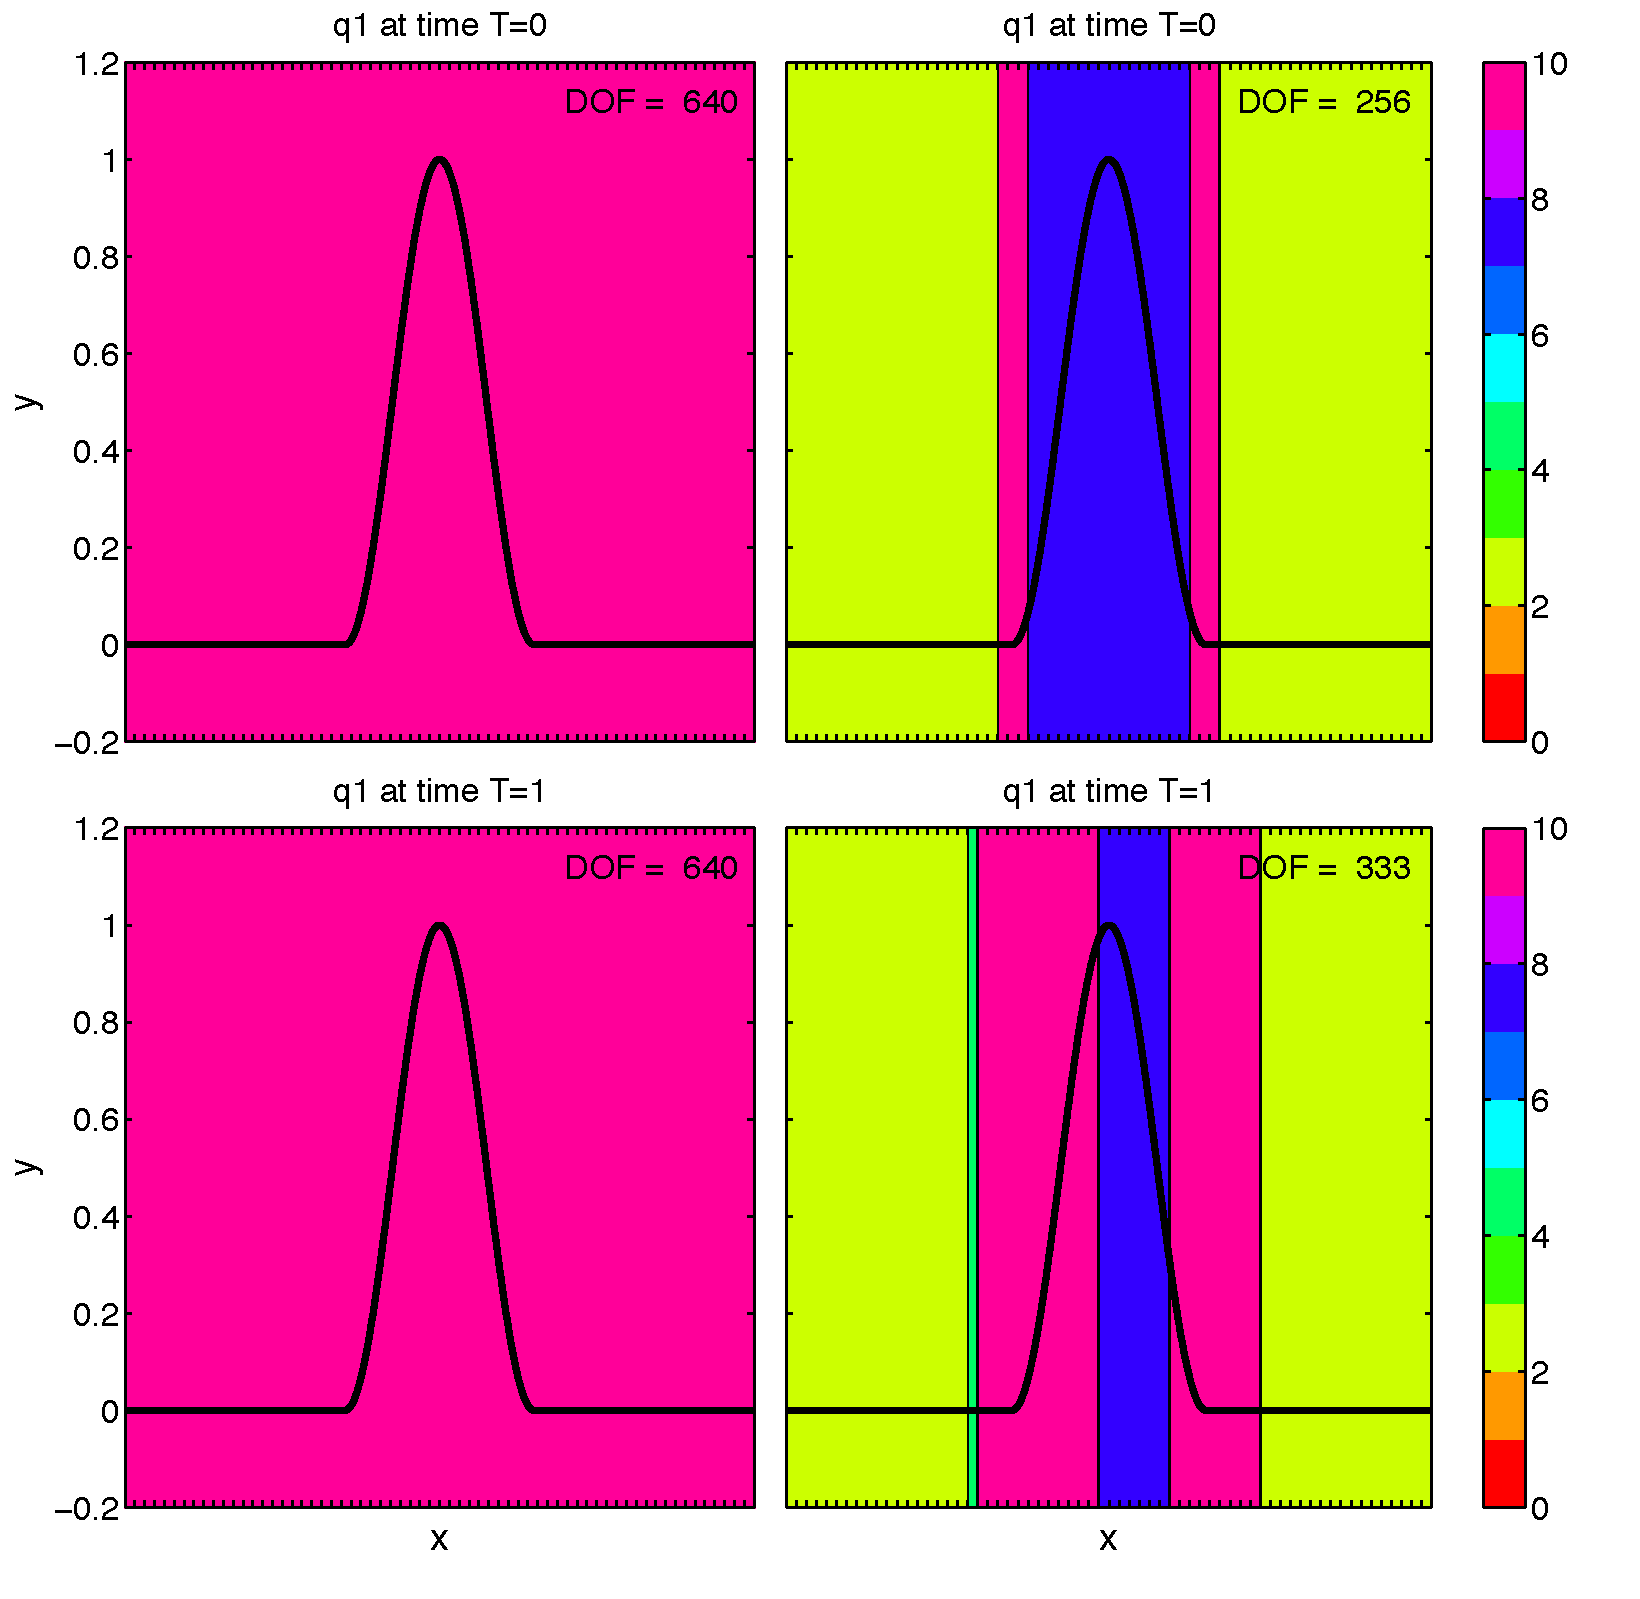
\includegraphics[width=4.0in]{figures/cosbellCmpre_E64N10.pdf}\hfil
\caption{Constant wind-speed ($\bar u = 1$) advection of a $C_0$ cosine bell over a periodic domain using $p_{max} = 10$ and $64$ cells. Initial conditions ( {\bf a)} and {\bf b)} ) and final solution ( {\bf c)} and {\bf d)} ) for standard DG and $p$-adaptive DG respectively. Colored regions indicate local polynomial degree truncation. Total degrees of freedom are listed in the top right corner. } \label{cosbellCmpre}
\end{figure}

The simplest hyperbolic PDE to simulate is the constant wind-speed advection 
\begin{equation*}
q_t + \bar{u} q_x  = 0.
\end{equation*}
In Figure \ref{cosbellCmpre} a $C_0$ cosine bell is advected with wind-speed $\bar{u} = 1$ over a periodic domain for one revolution. In the left panels a DGFEM with uniform degree $p_{max}$ is used to simulate the PDE while in the right panels the local polynomial degree is allowed to vary between cells up to $p_{max}$. The colors of each region indicate the reconstructing polynomial degree within that area. Away from the two kinks where the solution meets the horizontal axis the cosine bell is smooth and its Legendre series coefficients decay rapidly. This implies that the $p$-adaptive method is able to use a relatively small number of degrees of freedom in order to capture the solution in the smooth areas. However, in the remaining regions near the kinks the coefficients do not decay rapidly and it is beneficial to maintain a high degree approximation. Overall the adaptive method is able to produce a similarly accurate solution using roughly half the total degrees of freedom. Notice that the high degree 
regions in the $p$-adaptive solution tracks along the corners in the exact solution. 

We can examine an empirical convergence rate to the true solution as degrees of freedom are added to either method. Figure \ref{cosbellEfficiency} plots the $L_2$ error as a function of the total degrees of freedom used in the integration. Each point along either curve doubles the number of cells starting with $16$ (top left) and ending with $256$ (bottom right) cells. For a coarse number of cells the two methods use a similar number of degrees of freedom because each cell is responsible for approximating a larger portion of the exact solution so each cell contains a large amount of variation which keeps an increasing number of coefficients important. Notice that between runs with an equal number cells the two methods produce similarly accurate solutions but that the adaptive scheme uses progressively fewer (up to a factor of $1/3$) total degrees of freedom. This difference in degrees of freedom translates directly into a correspondingly sized difference in CPU time for the integration.

\begin{figure}
\hfil\includegraphics[width=3.25in]{figures/efficency.pdf}\hfil
\caption{Comparison of the $L_2$ error versus total degrees of freedom (DOF) for constant speed advection of a cosine bell using $p$-adaptive and non-adaptive DG methods. } \label{cosbellEfficiency}
\end{figure}

\subsection{Burger's Equation}
A significantly more challenging problem is given by Burger's equation:
\begin{equation*}
q_t + \left( \frac{q^2}{2}\right)_x = 0
\end{equation*}
In this case even smooth initial data can develop into shocks after some time. Figure \ref{burgersGaussian} illustrates the $p$-adapted DGFEM solution to Burger's equation with a steep (but smooth) Gaussian bump initial condition. After a short time the solution develops a shock and the local polynomial expansion gives a relatively poor approximation to the true solution. Thus we can expect our adaptive method to use the maximum degree polynomial allowed in these regions. However, away from the shock the solution remains smooth and a good approximation is obtained using many fewer polynomials. 

\begin{figure}
\hfil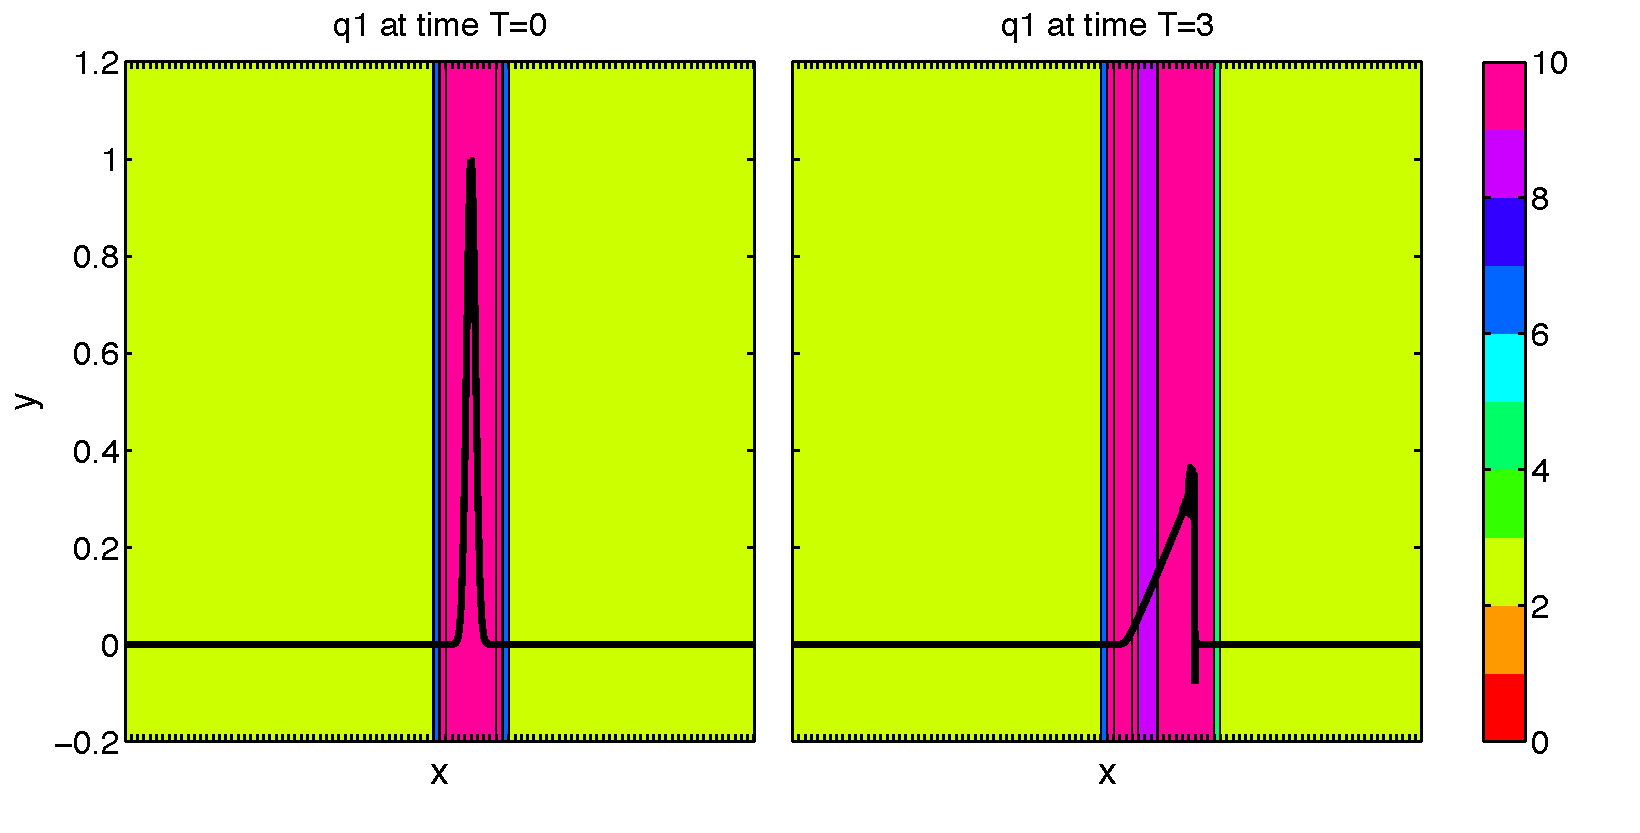
\includegraphics[width=5in]{figures/burgers_heat.pdf}\hfil
\caption{$p$-adaptive DG simulation of Burger's equation on a periodic domain using $64$ cells at {\bf a)} the initial time and {\bf b)} time $T=3$. Color indicates local polynomial degree. }
\label{burgersGaussian}
\end{figure}

\subsection{Acoustics}
Lastly we can consider our method applied to a non-conservative hyperbolic system 

\begin{equation*}
\begin{bmatrix}
P\\ u
\end{bmatrix}_t+\begin{bmatrix} 0 & c(x)^2 \rho(x) \\ \frac{1}{\rho(x)} & 0 \end{bmatrix}
\begin{bmatrix}
P \\ u
\end{bmatrix}_x
\end{equation*}
A similar problem is examined in Section 9.7 of the textbook. For this problem
we use an exact Riemann solver that accounts for the fact that there is not a flux function. Our Riemann solver
is constructed following section $9.9$ of the text.
Although we begin with a smooth initial condition, the exact solution is not continuously differentiable because of the jump in material properties. Figure \ref{variableAcoustics} illustrates the $p$-adaptive method just before and just after the pulse interacts with the interface. Even though the exact solution is not smooth near the interface the method only looks at coefficient decay locally in each cell. So the p-adaptive scheme continues to treat the solution as if it is a smooth function that has steepened.

\begin{figure}
\hfil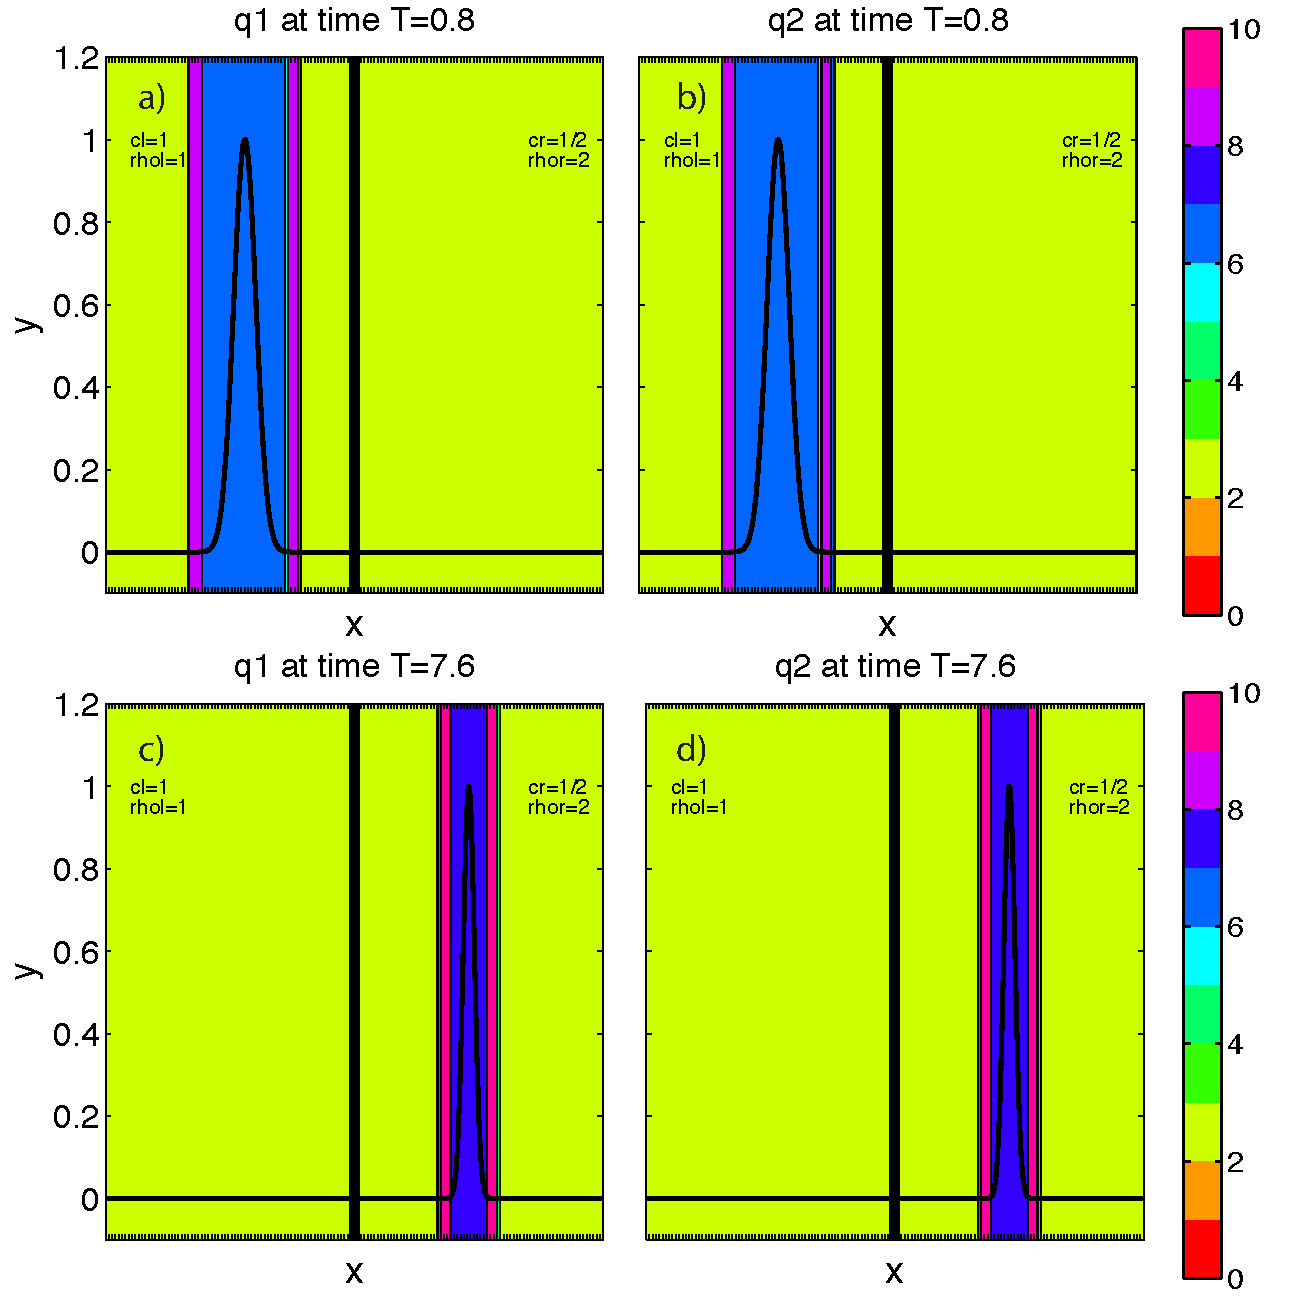
\includegraphics[width=4in]{figures/acousticVariableCoeff.pdf}\hfil
\caption{Right going acoustic gaussian pulse hitting an interface between two materials (thick vertical line) where the sound speed changes from $1$ to $0.5$ but the impedance remains unchanged. Left column $q_1$, right column $q_2$. }
\label{variableAcoustics}
\end{figure}

\subsection{Conclusion}
We have investigated a simple scheme for a local polynomial adaptive DGFEM. Our preliminary results show that this technique can be valuable in reducing the number of degrees of freedom required to obtain an accurate approximation for solutions with even moderate regularity. However, discontinuities present a serious challenge to any piecewise polynomial approximation and imply that limiting remains an important aspect of high order approximation. In order to further improve our method future work might focus on improving efficiency by implementing local time stepping, adaptive quadrature rules, and simultaneous $h$--$p$ refinement.

\newpage
\bibliographystyle{plain}
\bibliography{sources}
\end{document}